\documentclass[12pt,a4paper]{article}%шаблон для статьи, шрифт 12 пт
\usepackage[utf8x]{inputenc} %использование кодировки Юникод UTF-8
\usepackage[russian]{babel} %пакет поддержки русского языка
\usepackage[compact]{titlesec}%для titlespacing
\titlespacing*{\section}{0.75cm}{1em}{0.1em}%отступ заголовка
\titlespacing*{\subsection}{0.75cm}{1em}{0.1em}
\usepackage{indentfirst}%отступ первого абзаца
\setlength{\parindent}{0.75cm}
\usepackage[labelsep=endash]{caption}%тире вместо двоеточия в картинках
\usepackage{graphicx}%кртинки
\usepackage{color}%     цветной код
\usepackage{listings}%листинги кода из файлов



\begin{document}
	
	\thispagestyle{empty}
	
	\begin{center}
		\Large{
			\textbf{МИНОБРНАУКИ РОССИИ}
			
			\textbf{Санкт-Петербургский государственный}
			
			\textbf{электротехнический университет «ЛЭТИ»}
			
			\textbf{им. В.И. Ульянова (Ленина)}
			
			\textbf{Кафедра САПР}
		}
	\end{center}
	
	\topskip=0pt
	\vspace*{\fill}
	\begin{center}
		\Large{
			\textbf{
				ЛАБОРАТОРНАЯ РАБОТА №1\\
				по дисциплине «Программирование»\\
				Тема: Обработка массивов\\
			}
		}
	\end{center}
	\vspace*{\fill}
	
	\begin{tabular}{lcr}
		Студенты гр. 9892 & \begin{tabular}{p{60mm}} \\ \hline \end{tabular} & Лескин К.А.  \\\\
		                 & \begin{tabular}{p{60mm}} \\ \hline \end{tabular} & Миллер В.В. 
		\\\\
		Преподаватель    & \begin{tabular}{p{60mm}} \\ \hline \end{tabular} & Кузьмин С.А. 
		\\\\
	\end{tabular} 
	
	\begin{center}
		Санкт-Петербург\\
		2020
	\end{center}
	%////////////////////////////////////////////////////////////////////////////////////////////////
	%////////////////////////////////////////////////////////////////////////////////////////////////
	%////////////////////////////////////////////////////////////////////////////////////////////////
	\newpage
	
	\section*{Цель работы}
	
	Получение
	практических
	навыков
	разработки
	программы,
	обрабатывающей числовые данные, представленные в форме массива.
	
	\section*{Формулировка задания}
	
	Разработать
	программу,
	обрабатывающую
	элементы
	двумерного
	массива размером n × n, в соответствии с индивидуальным вариантом.
	Размерность
	массива
	n
	должна
	вводиться
	пользователем с клавиатуры (если среда выполнения программы это не
	позволяет, тогда данную размерность можно задать в программе заранее как
	константу). Элементы массива также должны вводиться пользователем с
	клавиатуры. Исходный и преобразованный массивы должны быть выведены
	на экран после обработки.
	
	Индивидуальный вариант: Умножить на заданное число.
	
	\ \\
	\ * * * -\\
	\ * * - -\\
	\ * - - -\\
	\ - - - -\\
	
	\section*{Описание структур данных}
	
	В лабораторной работе применятся технология хранения данных в виде двумерного массива.
	
	В общем случае двумерные массивы можно рассматривать как матрицы c $i$ строк и $j$ столбцов (рис. \ref{scheme})
	
	\begin{figure}[hpt!]
		\centering
		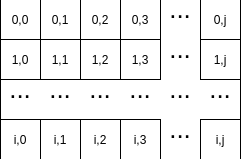
\includegraphics[width=0.6\linewidth]{scheme}
		\caption{Схема представления массива}
		\label{scheme}
	\end{figure}
	
	\section*{Алгоритм программы}
	
	\begin{itemize}
		\item Пользователю предлагается ввести размер массива (более 1)
		
		\item Предлагается выбор по заполнению массива
		
		\subitem Случайными числами
		
		В этом случае идёт проход по всему массиву и каждому элементу присваивается случайное число от -100 до 100.
		
		\begin{itemize}
			\item цикл по $i$ от 0 до $size$
			\subitem цикл по $j$ от 0 до $size$
			\subsubitem элементу $ (i,j) $ присваивается случайное число.
		\end{itemize}
		
		\subitem Единицами
		
		В этом случае идёт проход по всему массиву и каждому элементу присваивается 1.
		
		\begin{itemize}
			\item цикл по $i$ от 0 до $size$
			\subitem цикл по $j$ от 0 до $size$
			\subsubitem элементу $ (i,j) $ присваивается 1.
		\end{itemize}
		
		\subitem От 0 до размера массива
		
		В этом случае идёт проход по всему массиву и каждому элементу присваивается его порядковый номер по формуле $ i*size+j $
		
		\begin{itemize}
			\item цикл по $i$ от 0 до $size$
			\subitem цикл по $j$ от 0 до $size$
			\subsubitem элементу $ (i,j) $ присваивается $ i*size+j $
		\end{itemize}
		
		\subitem Вручную
		
		В этом случае идёт проход по всему массиву и каждому элементу присваивается значение, введённое с клавиатуры
		
		\begin{itemize}
			\item цикл по $i$ от 0 до $size$
			\subitem цикл по $j$ от 0 до $size$
			\subsubitem элементу $ (i,j) $ присваивается введённое с клавиатуры число
		\end{itemize}
		
		\item Выводится созданный массив
		\begin{itemize}
			\item цикл по $i$ от 0 до $size$
			\subitem цикл по $j$ от 0 до $size$
			\subsubitem элемент $ (i,j) $ выводится на экран, после знак табуляции
			\subitem Выводится знак переноса строки
		\end{itemize}
		
		\item С клавиатуры вводится число, на которое домножаются все элементы, определённые в индивидуальном задании
		
		\item Идёт обход массива по тем элементам, которые нужно домножить на заданное число
		
		\begin{itemize}
			\item цикл по $i$ от 0 до $size$
			\subitem цикл по $j$ от 0 до $size - 1 - i$
			\subsubitem элемент $ (i,j) $ домножается на заданное число
		\end{itemize}
		
		\item Выводится обработанный массив
		\begin{itemize}
			\item цикл по $i$ от 0 до $size$
			\subitem цикл по $j$ от 0 до $size$
			\subsubitem элемент $ (i,j) $ выводится на экран
			\subitem Выводится знак переноса строки
		\end{itemize}
		
	\end{itemize}
\newpage
	
	\section*{Тестирование программы}
	
	На рис. \ref{t1} представлен пример выполнения программы при заполнении массива 1. Так же в этом примере Произведена попытка ввести некорректное значение размера массива.
	
	На рис. \ref{t2} представлен пример выполнения программы при заполнении массива случайными числами.
	
	
	На рис. \ref{t3} представлен пример выполнения программы при заполнении массива порядковыми номерами.
	
	На рис. \ref{t4} представлен пример выполнения программы при заполнении массива вручную.
	
	\begin{figure}[hpt!]
		\centering
		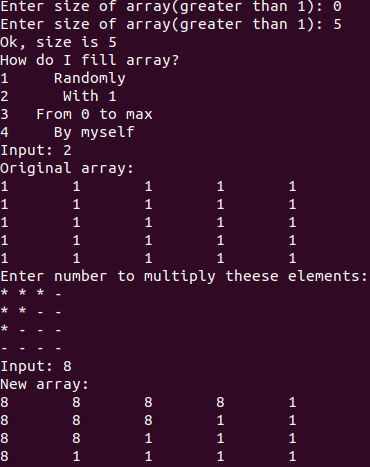
\includegraphics[width=0.6\linewidth]{t1}
		\caption{Пример 1}
		\label{t1}
	\end{figure}

	\begin{figure}[hpt!]
		\centering
		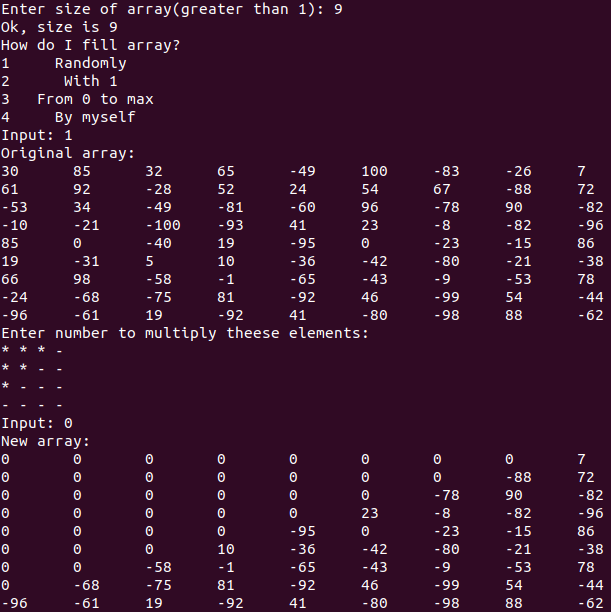
\includegraphics[width=0.6\linewidth]{t2}
		\caption{Пример 2}
		\label{t2}
	\end{figure}

	\begin{figure}[hpt!]
		\centering
		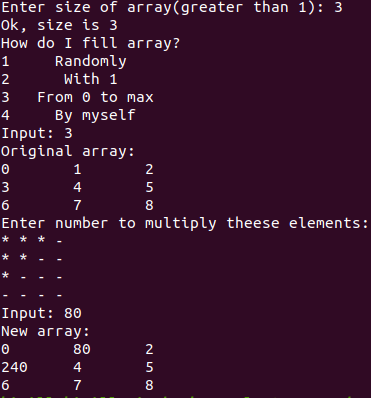
\includegraphics[width=0.6\linewidth]{t3}
		\caption{Пример 3}
		\label{t3}
	\end{figure}
	
	\begin{figure}[hpt!]
		\centering
		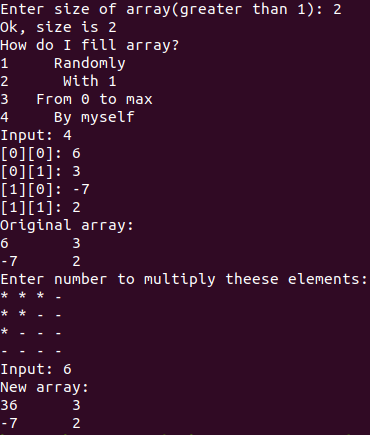
\includegraphics[width=0.6\linewidth]{t4}
		\caption{Пример 4}
		\label{t4}
	\end{figure}
	
	\newpage
	\section*{Выводы}
	
	В результате выполнения данной лабораторной работы мы закрепили и применили на практике знания, полученные в ходе изучения темы "Обработка массивов". Реализованная программа соответствует поставленным задачам и безошибочно выполняет свою работу. Функционал программы позволяет не только выполнять вычисления, но и реализует полноценное взаимодействие с пользователем, корректно обрабатывать его запросы и выдавать ему ожидаемый результат. Выполнение данной лабораторной работы позволило углубить наши знания в технологии программирования типовых задач обработки массивов.
	
	\newpage
	\section*{Приложение А. Листинг программного кода}
	\lstinputlisting{lr1.cpp}
\end{document}